\documentclass[a4paper,10pt]{report}
\usepackage[utf8]{inputenc}
\usepackage{graphicx}
\usepackage{here}

% Title Page
\title{FAA partie 1}
\author{Matthieu Caron}


\begin{document}
\maketitle

\section{TP 1 : Calcul de performance}

Voici les différents résultats obtenus avec les différentes mesures de performance.
$$J_{abs} = 0.73987984094 $$
$$J_{l1} = 0.0896787983772$$
$$J_{l2} = 0.804228687838$$
$$J_{l\infty} = 2.51624302238$$



\begin{figure}[H]
 \centering
 \caption{Comparaison entre $2*x + 3$ et les points générés}
 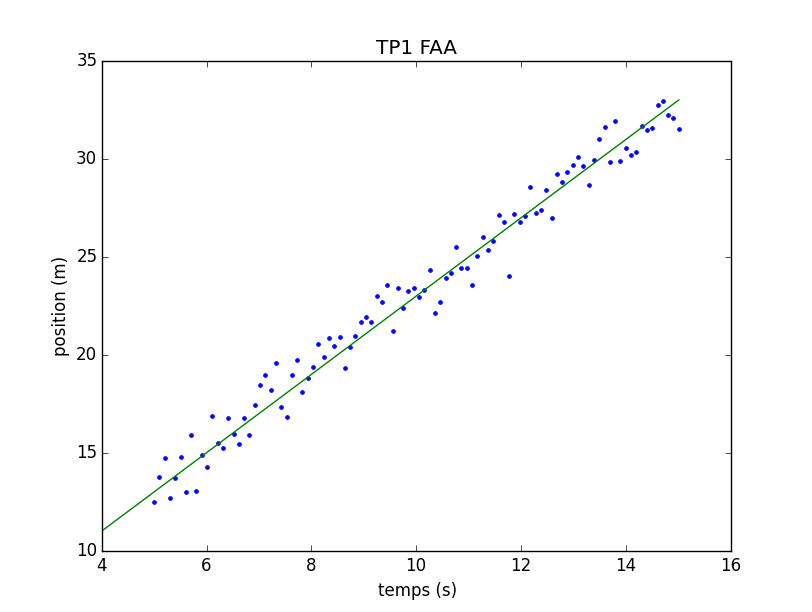
\includegraphics[width=10cm]{tp1.png}
\end{figure}

\section{TP 2 :  Moindres Carrés}
Les valeurs qui ont permis de générer les points sont 2 et 3 mais il existe un meilleur vecteur teta pour aproximer 
les points obtenus. Comme la fonction est une fonction linéaire on peut l'approximer avec les moindres carrés.
Notre fonction $2*x+3$ devient maintenant : $$1.95293789 * x + 3.59623499 $$

\begin{figure}[H]
 \centering
 \caption{Nouvelle approximation}
 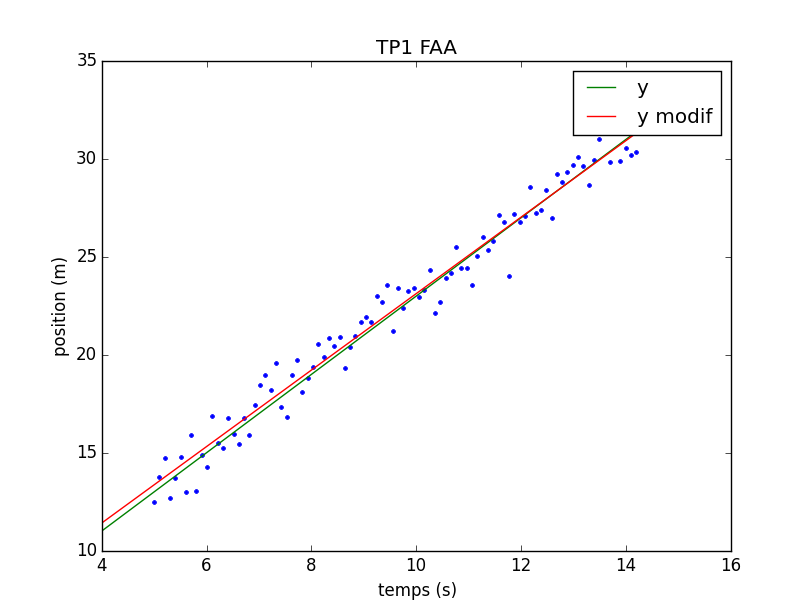
\includegraphics[width=10cm]{tp2.png}
\end{figure}

Voici les résultats des mesures de performance après les moindres carrés.
$$J_{abs} = 0.727356264922$$
$$J_{l1} = 0.0877279862436 $$
$$J_{l2} = 0.769619957035$$
$$J_{l\infty} = 2.55866627298$$

Et enfin les différences avec les résultats du tp1.

$$diff(J_{abs}) =  0.0125235760181$$
$$diff(J_{l1}) = 0.00195081213361$$
$$diff(J_{l2}) =  0.0346087308024$$
$$diff(J_{l\infty}) = 0.0424232506015$$

\section{TP 3 : Descente de gradient }
J'ai implémenté la descente de gradient globale qui évalue donc tout le jeu de donné avant d'apprendre et 
j'ai aussi implémenté la descente de gradient stochastique qui évalue une donné au hasard et apprend tout de suite après.
Comme on peut l'observer sur les figures, la descente stochastique est bruité. 
J'ai aussi fait varier le pas d'apprentissage alpha de la forme $\alpha = \frac{1}{i*100+t}$ en fonction de i et voici le résultat.
\begin{figure}[H]
 \centering
 \caption{Descente de gradient globale}
 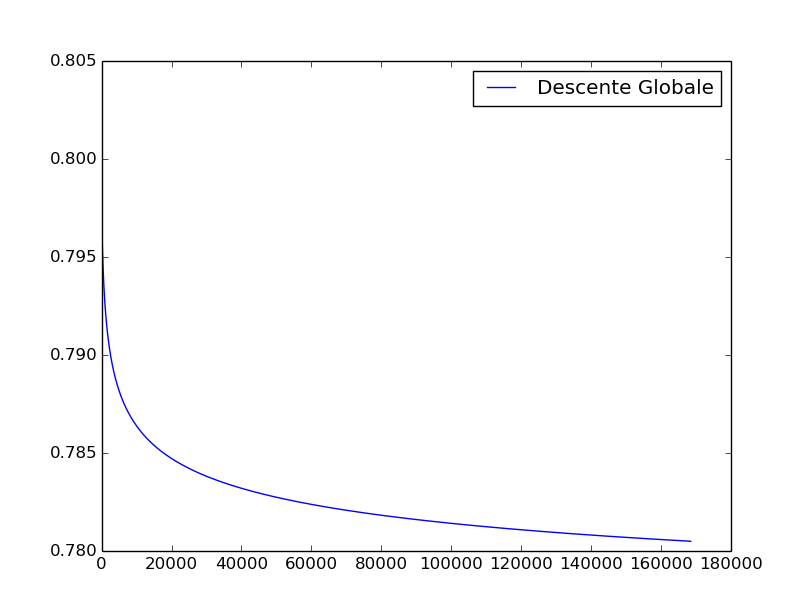
\includegraphics[width=10cm]{globale.png}
\end{figure}

\begin{figure}[H]
 \centering
 \caption{Descente de gradient stochastique}
 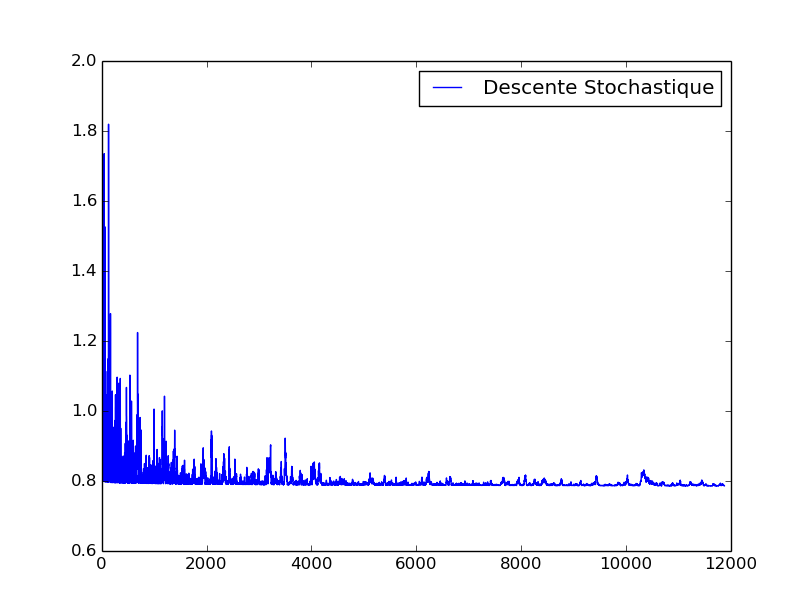
\includegraphics[width=10cm]{stochastique.png}
\end{figure}

\begin{figure}[H]
 \centering
 \caption{Differents départs pour alpha}
 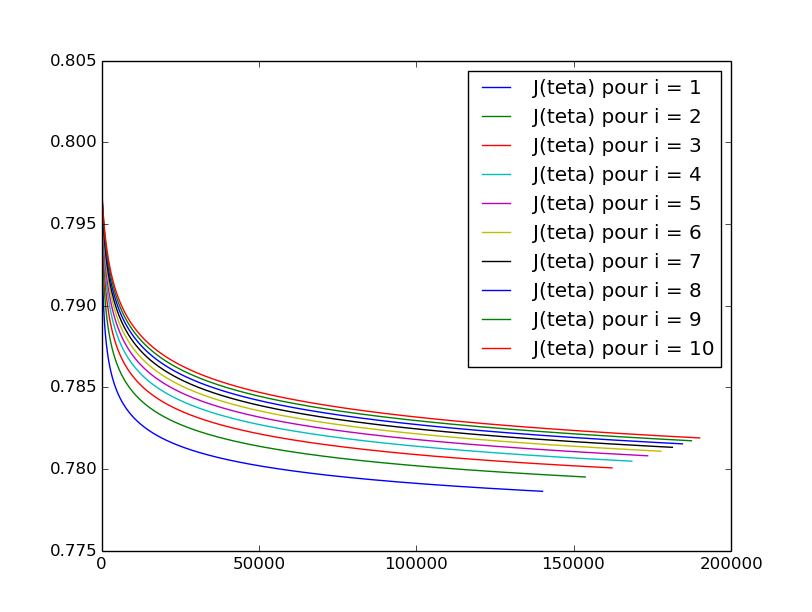
\includegraphics[width=10cm]{tp3.png}
\end{figure}

\section{TP4 : Généralisation et sur apprentissage}
Avec la méthode des moindres carré il est possible d'approximer des ensembles de points comme on peut l'observer si dessous,
cependant en machine learning il existe le phénomène de sur apprentissage c est a dire qu'on perd toute notion de prédiction,
qu'une fois sorti du set d'apprentissage on ne déduit pas la bonne valeur. Pour vérifier que l'on a pas sur-appris
on fait de la cross-validation, en général on garde 10 pour cent des données pour vérifier si on arrive a prédire les bonnes 
valeurs après apprentissage.

\begin{figure}[H]
 \centering
 \caption{matrix0}
 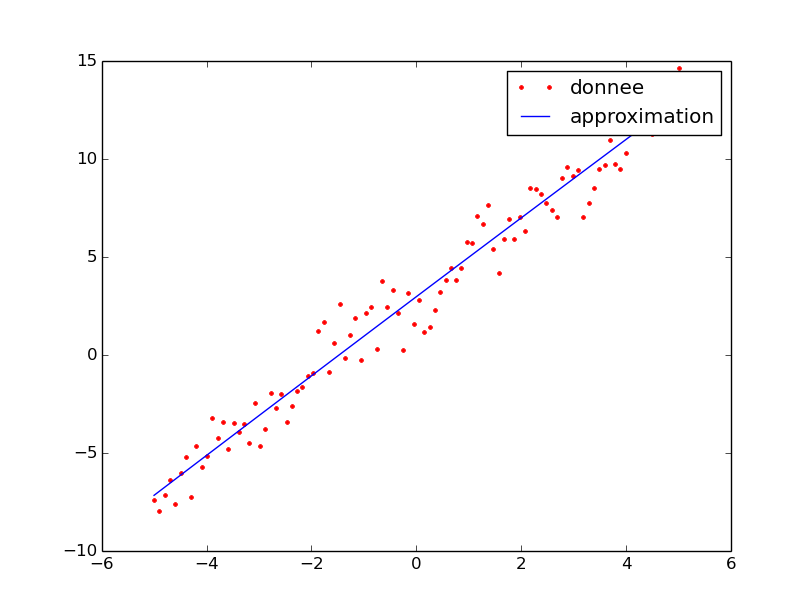
\includegraphics[width=10cm]{matrix0.png}
\end{figure}

\begin{figure}[H]
 \centering
 \caption{matrix1}
 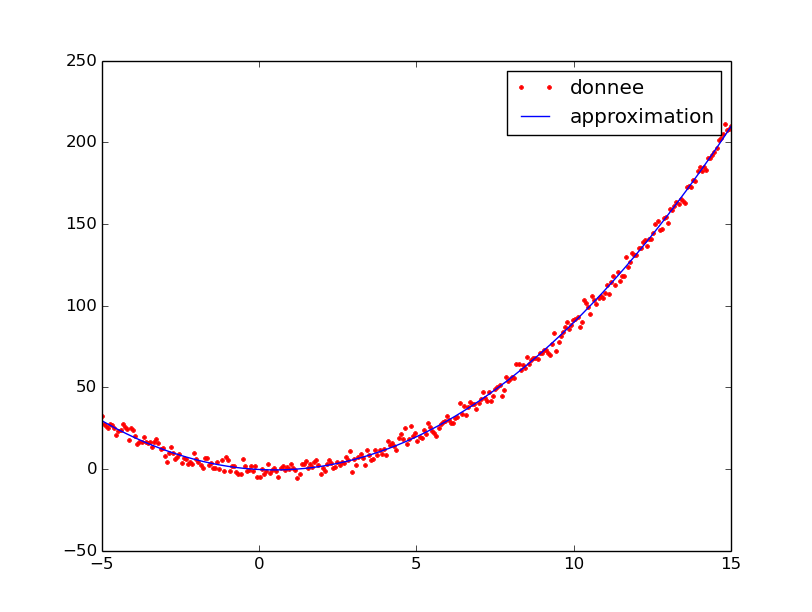
\includegraphics[width=10cm]{matrix1.png}
\end{figure}

\begin{figure}[!h]
 \centering
 \caption{matrix2}
 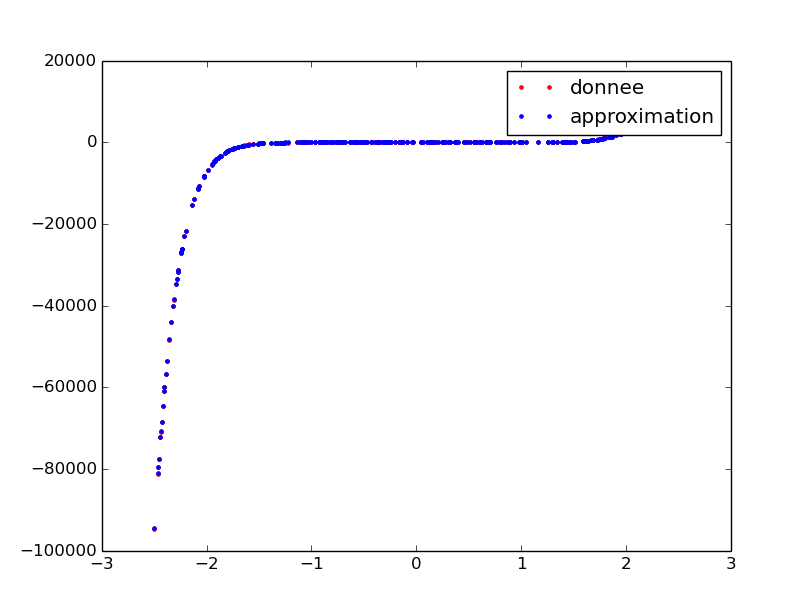
\includegraphics[width=10cm]{matrix2.png}
\end{figure}

\end{document}          
